\section*{Testdesign}
%
Til testen anvendes en visuel prototype af robotten, som er illustreret på \autoref{fig:position}. Testpersonerne bliver præsenteret for de fire forskellige hovedepositioner; position 1, som er 100$^{\circ}$, position 2, som er 65$^{\circ}$, position 3, som er 35$^{\circ}$, samt position 4, som er 0$^{\circ}$. De fire forskellige positioner er præsenteret på \autoref{fig:position}.   
%
\begin{figure}[H]
\centering
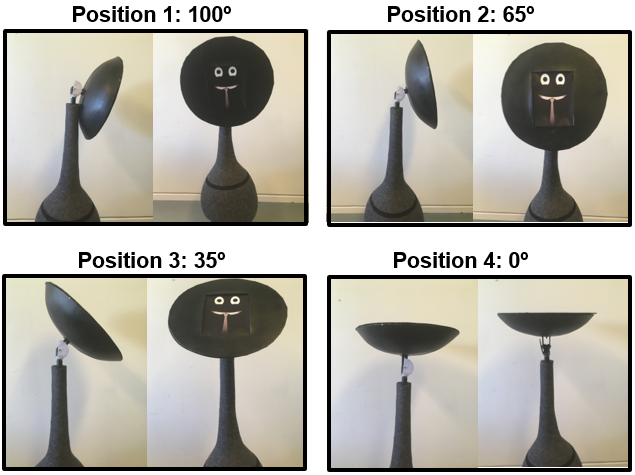
\includegraphics[width = \textwidth]{Figure/positionerBilleder.PNG} 
\caption{De fire valgte hovdepositioner.}
\label{fig:position}
\end{figure}
\noindent 
%
For at balancere stimulipræsentationen anvendes et \textit{Latin Square Design}, hvilket giver fire mulige kombinationer hvorved stimuli præsenteres i. Stimuli defineres som værende robottens hovedposition. For at indsamle mere data bliver hver kombinationsmulighed præsenteret to gange, hvilket medfører at der i alt vil blive indsamlet data fra otte testpersoner. Præsentationsrækkefølgen fremgår af \autoref{tab:Latin}.  
%
\begin{table}[H]
	\centering
	\begin{tabular}{l|c}
		Testperson     & Præsentationsrækkefølge for position \\\hline
		Testperson 1   & 1 - 2 - 3 - 4          \\\hline
		Testperson 2   & 2 - 3 - 4 - 1          \\\hline
		Testperson 3   & 3 - 4 - 1 - 2          \\\hline
		Testperson 4   & 4 - 1 - 2 - 3          \\\hline
		Testperson 5   & 1 - 2 - 3 - 4          \\\hline
		Testperson 6   & 2 - 3 - 4 - 1          \\\hline
		Testperson 7   & 3 - 4 - 1 - 2          \\\hline
		Testperson 8   & 4 - 1 - 2 - 3   
	\end{tabular}
	\caption{Præsentationsrækkefølgen for robottens fire hovedpositioner.}
	\label{tab:Latin}         
\end{table}
\noindent
%
Testen afvikles i forhallen på Frederik Bajers vej 7H, for at simulere et befolket område som eksempelvis en lufthavn. Dog udføres den ene af de to pilot tests i kantinen på Frederik Bajers vej 7.
%
\subsection*{Instruktioner}
\label{Instruktioner}
%
Testpersonerne får følgende instruktioner: 
%
\begin{quotation}
\noindent
Hej!\blankline
%
Fedt at du gider at hjælpe os. Du skal forestille dig, at det her er en robot. Lige nu kan den ingenting. Det er meningen at robotten skal indgå i en lufthavn, hvor der er mange mennesker. Hovedet vil blive indstillet i fire forskellige positioner og du skal derfra angive, hvor indbydende du synes robotten er. Det gør du på en skala fra slet ikke til ekstremt indbydende.\blankline
%
Har du nogen spørgsmål?
\end{quotation}
%
Derefter præsenteres testpersonen for de fire forskellige hovedpositioner i den specifikke rækkefølge, jævnfør \autoref{tab:Latin}. Efter hver præsentation udleveres en skala hvorpå testpersonen, med en kuglepen, angiver hvor indbydende de synes robotten var i netop den position.  
%

\subsection*{Design af skala}
%
Testpersonerne bliver til hver af de fire hovedpositioner spurgt om: \textit{Hvor indbydende synes du robotten er?}, hvortil testpersonerne angiver sin respons på en \textit{Visual Analog Scale} (VAS). Skalaen er opstillet med åbne endepunkter samt to ankerpunkter placeret 1,5 cm fra hvert endepunkt, skalaen er illustreret på \autoref{fig:VAS}. Venstre ankerpunkt er angivet med \textit{Slet ikke}, modsat det højre ankerpunkt, som er angivet med \textit{Ekstremt}. Ved at vælge en VAS med åbne endepunkter har testpersonerne mulighed for, at overgå sig selv i tilfælde af, at de perciperer robotten som værende endnu mere indbydende end den mest indbydende robot de hidtil har været udsat for. Ved at designe skalaen med åbne endepunkter undgåes ophobning af respons omkring endepunkterne. 
%
\begin{figure}[H]
\centering
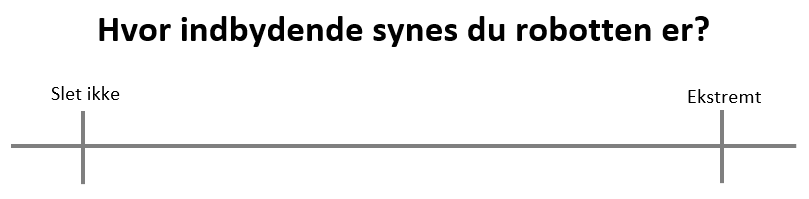
\includegraphics[width = 0.8\textwidth]{Figure/VAS.PNG} 
\caption{Illustration af den designede VAS med åbne endepunkter og med de angivne ankerpunkter, samt spørgsmålet som testpersonerne skal svare på.}
\label{fig:VAS}
\end{figure}
\noindent 
%